%
% body.tex
%
% Copyright © 2020 Libao Jin <jinlibao@outlook.com>
% Distributed under terms of the MIT license.
%
\ifx\undefined\sol
Submissions without signature will not be considered. All your work and this signed page should be together as one PDF file.
\vspace{3em}
\else
{ \large
\textbf{Honesty Clause: {\color{red}I hereby testify that all the work on this project is \underline{solely my own}. I have complied with the academic honesty guidelines as stated in the University regulations.}}

% \special{pdf:ann width 3in height 1in
%   <<
%     /T (My Signature)
%     /Subtype /Widget
%     /FT /Sig
%     /F 4
%     /Q 1
%     /MK << /BC [] >>
%   >>
% }

\begin{Form}
\TextField[width=21em,
           name = print.name,
           format = {
               var f = this.getField('print.name');
               % f.textFont = 'Verdana';
               % f.strokeColor = ['T'];
               % f.fillColor = ['T'];
               f.userName = 'Print Name'
               },
           value = ,
           charsize = 12pt]
          {Name: }
\end{Form}
\begin{Form}
\TextField[width=10em,
           format   ={AFDate_FormatEx("mm/dd/yyyy");},
           keystroke={AFDate_KeystrokeEx("mm.dd.yyyy");},
           value = ,
           charsize = 12pt]
           {Date: }
\end{Form}
}
\vspace{5em}
\fi

\textbf{Instruction}

\begin{enumerate}[label={\arabic*.}]
  \item Go to \url{https://www.overleaf.com} and sign in (required).
  \item Open \href{https://www.overleaf.com/read/jkcmttjccbdc}{template}, click \emph{Menu} (up left corner), then \emph{Copy Project}.
  \item Go to \verb|LaTeX/meta.tex| (the file \verb|meta.tex| under the folder \verb|LaTeX|) to change the section and your name, e.g.,
    \begin{itemize}
      \item change author to \verb|\author{Carl F. Gauss}|
    \end{itemize}
  \item You need to write function/script files, store results to output/plot files. Here are suggested names for function files, script files, output files, and plot files:
    \begin{table}[!hbtp]
      \centering
      \begin{tabular}{cllll}
        \toprule
        Problem & Function File                    & Script File                   & Output File         & Plot File               \\
        \midrule
        1       & \verb|cubic_spline.m|            & \verb|final_p1.m|             & \verb|final_p1.txt| & \verb|final_p1a.pdf|    \\
        1       &                                  &                               &                     & \& \verb|final_p1b.pdf| \\
        2       & \verb|backward_euler.m|       & \verb|final_p2.m|             &                     & \verb|final_p2.pdf|     \\
        3       & \verb|golden_section.m|          & \verb|final_p3.m|             & \verb|final_p3.txt| & \verb|final_p3.pdf|     \\
        3       & \& \verb|successive_parabolic.m| &                               &                     &                         \\
        \bottomrule
      \end{tabular}
    \end{table}

    Once finished, you need to upload these files to the folder \verb|src| on Overleaf. If you have different filenames, please update the filenames in \verb|\lstinputlisting{../src/your_script_name.m}| accordingly. You can code in the provided files in \href{https://libaoj.in/courses/2021s/MATH3340/final.zip}{final.zip}, and use the MATLAB script \verb|save_results.m| to generate the output files and store the graphs to \verb|.pdf| files automatically (the script filenames should be exactly same as listed above).
  \item Recompile, and download the generated \verb|.pdf| file.
  \item \textbf{\color{red}{Important}}: \underline{Enter your name and the date} in the above boxes \emph{before} you submit it on WyoCourses.
\end{enumerate}

\ifx\undefined\sol
\newpage
\fi

%%%%%%%%%%%%%%%%%%%%%%%%%%%%%%%%%%%%%%%%%%%%%%%%
% Problem 1
%%%%%%%%%%%%%%%%%%%%%%%%%%%%%%%%%%%%%%%%%%%%%%%%
\section{Problem 1}%
\label{sec:problem_1}
Consider the data in the following table:
\begin{table}[!hbtp]
  \centering
  \begin{tabular}{ccccc}
    \toprule
    $k$     & $0$   & $1$          & $2$          & $3$         \\
    \midrule
    $x_{k}$ & $0.0$ & $1.761062$   & $3.522123$   & $5.283185$  \\
    $y_{k}$ & $1.0$ & $-0.1891196$ & $-0.9284676$ & $0.5403023$ \\
    \bottomrule
  \end{tabular}
\end{table}

The values of $y$ in this table have been obtained as $y_{k} = \cos(x_{k})$. Your goal will be to create two different spline interpolants using these data points, and compare them with the original function.

\begin{enumerate}[label=(\alph*)]
  \item \label{enum:1a} Compute the usual spline interpolant $^{1} S(x)$ that uses the natural boundary conditions. Plot this interpolant versus the original function $\cos(x)$ using $100$ data points equally spaced between $x_{0}$ and $x_{3}$; make sure to also indicate the four data points on the plot using a special marker (you may use $\ast$ or $\circ$ for example).
  \item You will probably agree that the comparison at point \ref{enum:1a} above doesn't look very good. This is due to the fact that the natural boundary conditions do not match the behavior of the $\cos(x)$ function. Your task for this point is to modify your code to account for the correct second derivatives at the end points. In other words, create a new interpolant $^{2} S(x)$ that satisfies the following conditions:
    \begin{equation*}
      ^{2} S''(x_{0}) = -\cos(x_{0});
      \quad
      ^{2} S''(x_{3}) = -\cos(x_{3}).
    \end{equation*}
    You can do this by modifying the system of equations for the spline coefficients accordingly. Plot again the newly-obtained interpolant versus the original function in the same manner as above. Turn in your codes together with the two plots.
\end{enumerate}
\begin{solution}
  \quad
  \begin{itemize}
    \item Output file \verb|final_p1.txt|:
      \lstinputlisting[style=Plain]{../src/final_p1.txt}
    \item Plot files \verb|final_p1a.pdf| and \verb|final_p1b.pdf|:
      \begin{figure}[!hbtp]
        \centering
        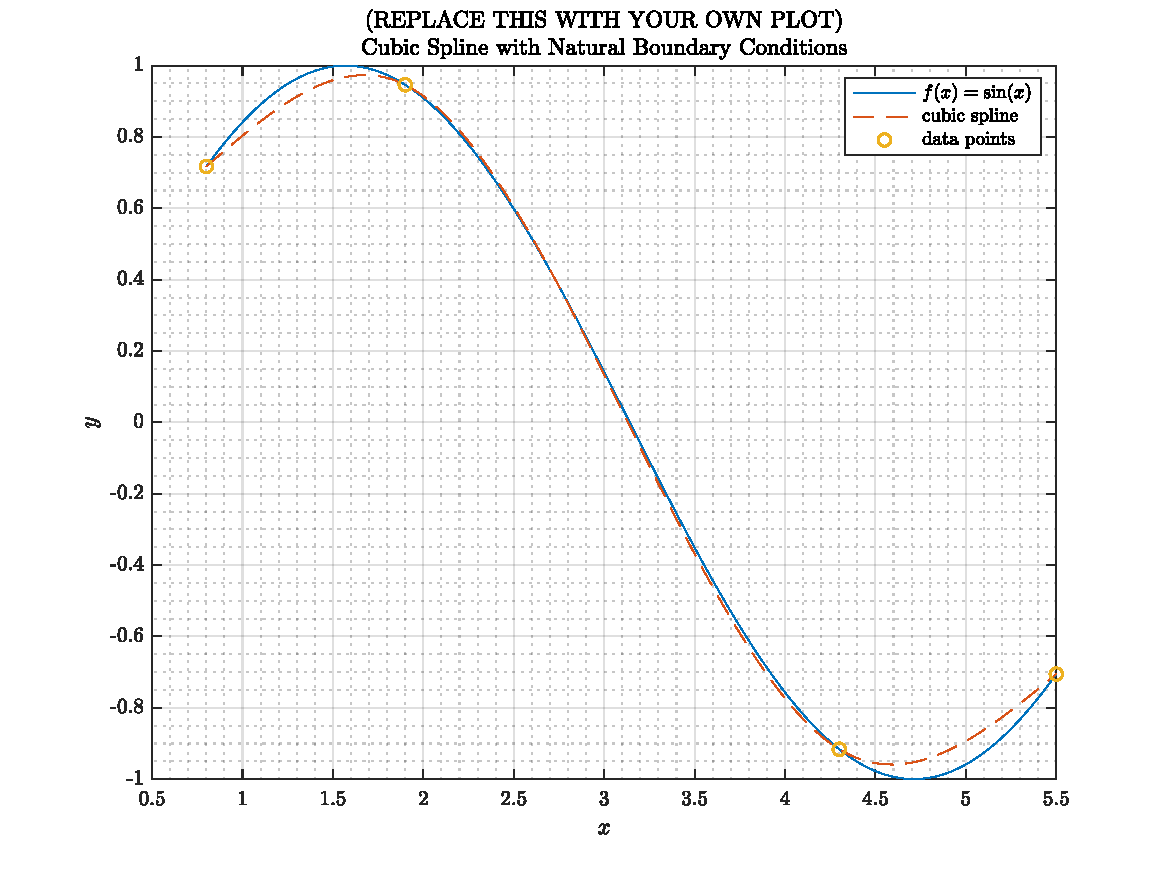
\includegraphics[width=0.8\textwidth]{../src/final_p1a.pdf}
        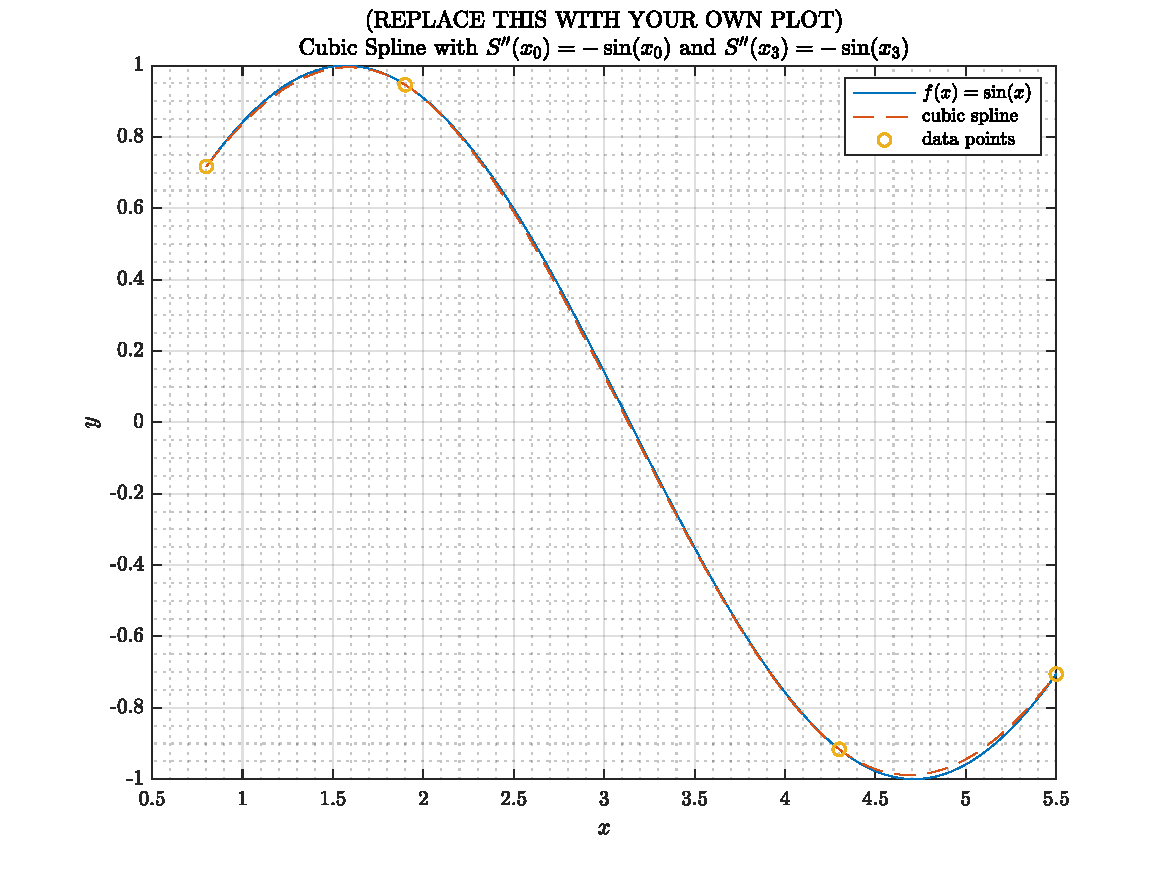
\includegraphics[width=0.8\textwidth]{../src/final_p1b.pdf}
        \caption{Cubic Spline With Different Boundary Conditions}
        \label{fig:p1}
      \end{figure}
    \newpage
    \item Function file \verb|cubic_spline.m|:
      \lstinputlisting[style=MATLAB]{../src/cubic_spline.m}
    \item Script file \verb|final_p1.m|:
      \lstinputlisting[style=MATLAB]{../src/final_p1.m}
  \end{itemize}
\end{solution}

%%%%%%%%%%%%%%%%%%%%%%%%%%%%%%%%%%%%%%%%%%%%%%%%
% Problem 2
%%%%%%%%%%%%%%%%%%%%%%%%%%%%%%%%%%%%%%%%%%%%%%%%
\section{Problem 2}%
\label{sec:problem_2}
The implicit, backward Euler method for the general first order initial value problem
\begin{equation*}
  \frac{du}{dt} = f(u, t), \quad u(t_{0}) = u_{0}
\end{equation*}
is given by
\begin{equation*}
  u_{n + 1} = u_{n} + (t_{n + 1} - t_{n}) f(u_{n + 1}, t_{n + 1}), \quad n = 0, 1, \ldots
\end{equation*}
Use this method to solve numerically the differential equation
\begin{equation*}
  \frac{du}{dt} = 2 + \sqrt{u - 2t + 3}
\end{equation*}
subject to the initial condition $u(0) = 1$. Use a constant time step $\Delta t = t_{n + 1} - t_{n} = 0.05$ and advance the solution to $t = 2$. Turn in the code and the plot of $u(t)$ versus $t$. On the plot, compare your numerical solution with the exact solution $u(t) = 1 + 4t + t^{2} / 4$. Use markers to highlight the points produced by the numerical solution.

\textbf{NOTE:} You will need to solve a nonlinear equation at each time step. Solutions that do not perform this task as required will not receive credit.
\begin{solution}
  \quad
   \begin{itemize}
    \item Plot file \verb|final_p2.pdf|:
      \begin{figure}[!hbtp]
        \centering
        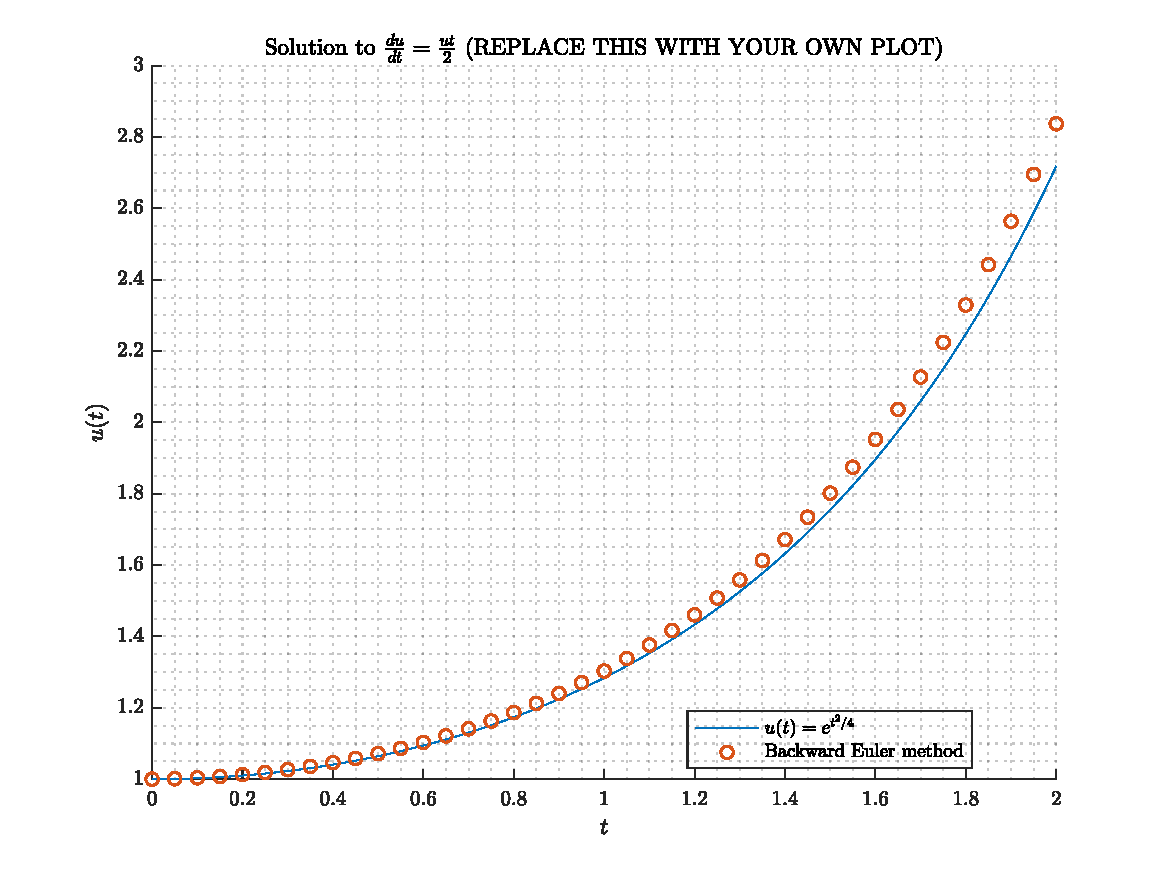
\includegraphics[width=0.8\textwidth]{../src/final_p2.pdf}
        \caption{Solution to $du / dt = 2 + \sqrt{u - 2t + 3}$ using Implicit Backward Euler Method}
        \label{fig:}
      \end{figure}
    \item Function file \verb|backward_euler.m|:
      \lstinputlisting[style=MATLAB]{../src/backward_euler.m}
    % UNCOMMENT THE NEXT TWO LINES IF YOU HAVE OTHER AUXILLIARY FUNCTIONS
    % \item Function file \verb|auxilliary_function.m|:
    %   \lstinputlisting[style=MATLAB]{../src/auxilliary_function.m}
    \item Script file \verb|final_p2.m|:
      \lstinputlisting[style=MATLAB]{../src/final_p2.m}
  \end{itemize}
\end{solution}

%%%%%%%%%%%%%%%%%%%%%%%%%%%%%%%%%%%%%%%%%%%%%%%%
% Problem 3
%%%%%%%%%%%%%%%%%%%%%%%%%%%%%%%%%%%%%%%%%%%%%%%%
\section{Problem 3}%
\label{sec:problem_3}
Use both successive parabolic interpolation and the golden section search method to find the minimum of the function $f(x) = |x^{2} - 2| + |2x + 3|$ on the interval $[-4, 0]$ with a tolerance of $10^{-8}$ and an identical accuracy. You are again requested to do this with MATLAB codes which you must show, together with the output; recall that golden search method code was discussed in detail in class. For parabolic interpolation, remember that some approximation steps may produce points that are not feasible and must be replaced. Write your code such that it reverts to the golden section search in that case.

\begin{solution}
  \quad
  \begin{itemize}
    \item Output file \verb|final_p3.txt|:
      \lstinputlisting[style=Plain]{../src/final_p3.txt}
    \item Plot file \verb|final_p3.pdf|:
      \begin{figure}[!hbtp]
        \centering
        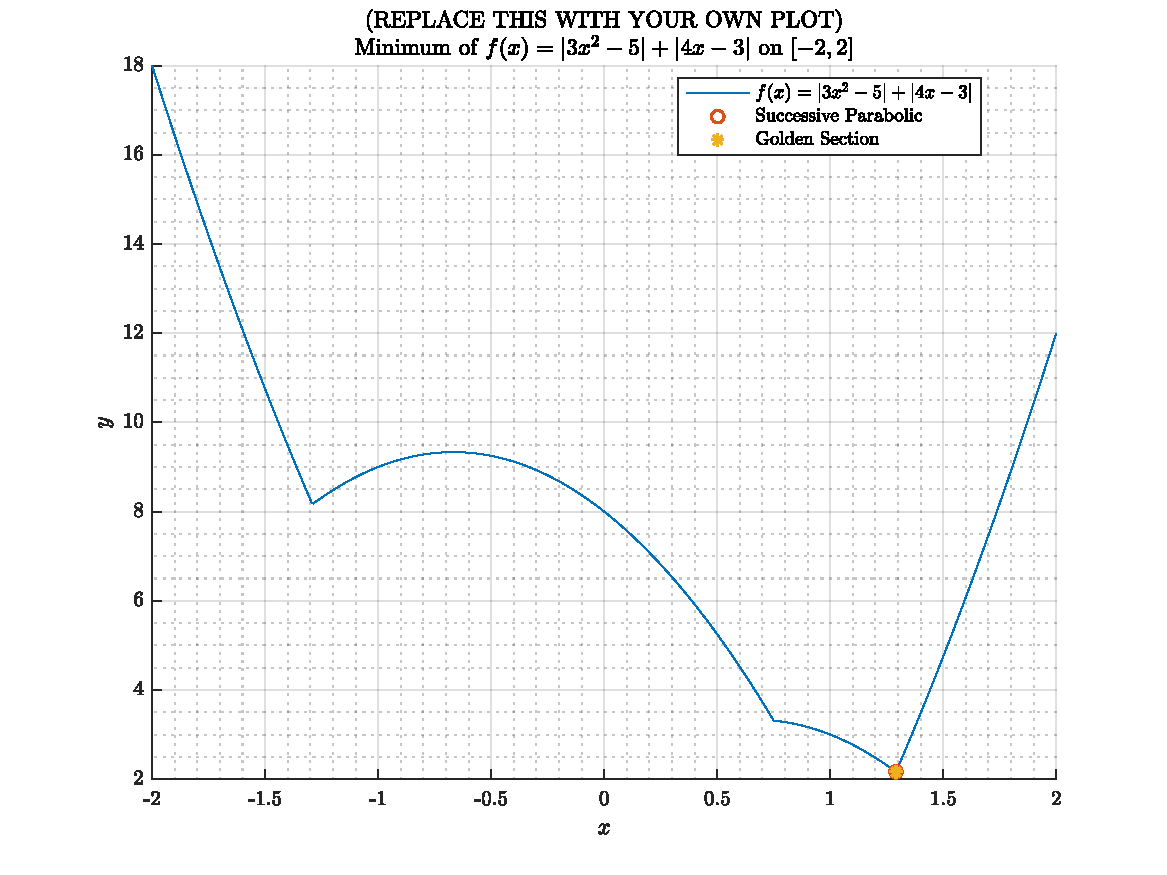
\includegraphics[width=0.8\textwidth]{../src/final_p3.pdf}
        \caption{Minimum Obtained by Successive Parabolic Interpolation and Golden Section Search Method}
        \label{fig:}
      \end{figure}
    \item Function file \verb|successive_parabolic.m|:
      \lstinputlisting[style=MATLAB]{../src/successive_parabolic.m}
    \item Function file \verb|golden_section.m|:
      \lstinputlisting[style=MATLAB]{../src/golden_section.m}
    \item Script file \verb|final_p3.m|:
      \lstinputlisting[style=MATLAB]{../src/final_p3.m}
  \end{itemize}
\end{solution}
